\section{Дървета на извод}

\tikzset{
  photon/.style={decorate, decoration={snake}, draw=black}
}

\marginpar{Понятието дърво е едно от най-основните в информатиката и може да се дефинира по много различни начини, в зависимост от това за какви цели се използва. Тук на практика следваме \cite{nerode-shore}, защото е важно да имаме наредба между възлите на дървото.}
\begin{itemize}
\item
  За всеки две думи $\alpha$ и $\beta$ над $\{0,1,\dots,b-1\}$, с $\alpha \preceq \beta$ ще означаваме, че $\alpha$ е префикс на $\beta$.
\item
  \index{наредба!лексикографска}
  За две думи $\alpha$ и $\beta$ над $\{0,1,\dots,b-1\}$ ще казваме, че $\alpha$ е лексикографски по-малка от $\beta$, което ще означаваме като $\alpha <_{\texttt{lex}} \beta$, ако
  \[(\exists i < \min\{|\alpha|,|\beta|\})[\ (\forall j < i)[\ \alpha[j] = \beta[j]\ ]\ \&\ \alpha[i] < \beta[i]\ ].\]
\item
  \index{дърво}
  \marginpar{Всеки възел в дървото еднозначно се определя от пътя от възела до корена.}
  Непразното множество $T \subseteq \{0,1,\dots,b-1\}^\star$ се нарича {\bf дърво},
  ако $T$ е затворено относно префикси, т.е. $\texttt{Pref}(T) = T$.
  С други думи,
  \[(\forall \alpha, \beta)[\ \alpha \in T\ \&\ \beta \preceq \alpha\ \implies\ \beta \in T\ ].\]
  \marginpar{При нас всички дървета са крайно разклонени.}
\item
  Нека да въведем следните означения:
  \begin{align*}
    & \texttt{height}(T) \df \max\{\ \abs{\alpha}\ \mid\ \alpha \in T\ \} & \comment\text{височина}\\
    & \texttt{ext}_T(\alpha) \df \{ \alpha i \mid \alpha i \in T\ \&\ i < b\} & \comment\text{наследниците на }\alpha\\
    & T_\alpha \df \alpha^{-1}(T) & \comment\text{поддървото на }\alpha\\
    & \texttt{front}(T) \df \{ \alpha \in T \mid \texttt{ext}_T(\alpha) = \emptyset \}. & \comment\text{листата на }T
  \end{align*}

  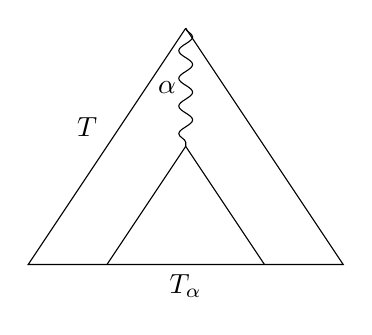
\begin{tikzpicture}
    \coordinate (A) at (0,0);
    \coordinate (B) at (-2,-3);
    \coordinate (C) at (2,-3);
    \coordinate (D) at (0,-1.5);
    \coordinate (E) at (-1,-3);
    \coordinate (F) at (1,-3);
    \draw (A) -- node[above left]{$T$} (B) -- node[below]{$T_\alpha$}(C) -- (A);
    \draw (D) -- (E);
    \draw (D) -- (F);
    \draw [photon] (A) -- node[left]{$\alpha$} (D);
  \end{tikzpicture}
\item
  Нека фиксираме граматиката $G = (\Sigma,V,S,R)$.
  С всяко дърво $T$ ще асоциираме функцията $\lambda: T \to V \cup \Sigma \cup \{\varepsilon\}$.
  Нека положим $X_\alpha \df \lambda(\alpha)$.
\item
  \index{дърво на извод}
  \marginpar{Също се нарича синтактично дърво. На англ. \emph{parse tree}.}
  Двойката $P = (T,\lambda)$ се нарича {\bf дърво на извод} съвместимо с $G$, ако са изпълнени свойствата:
  \begin{itemize}
  \item
    $T$ е крайно.
  \item
    Ако $\alpha i \in T$, то $\alpha j \in T$ за всяко $j < i$.
  \item
    Ако $\alpha \in T$ и $|\texttt{ext}_T(\alpha)| = k+1$, за някое $k \in \Nat$, то $X_\alpha \in V$,
    като имаме също така и 
    % Освен това, ако $\alpha_0,\dots,\alpha_k$ са всички думи от множеството $\texttt{ext}_T(\alpha)$
    % подредени във възходящ ред относно лексикографската наредба, то имаме, че:
    \marginpar{С други думи,
      \[\lambda(\alpha)\to_G\lambda(\alpha 0)\cdots\lambda(\alpha k).\]}
    \[X_\alpha \to_G X_{\alpha 0} X_{\alpha 1} \cdots X_{\alpha k}.\] 
  \end{itemize}
\item
  За дървото на извод $P$, нека
  \[\texttt{root}(P) \df X_\varepsilon.\]
\item
  Нека $\alpha_0, \alpha_1,\dots,\alpha_k$ са всички думи от множеството $\texttt{front}(T)$
  подредени във възходящ ред относно лексикографската наредба. Тогава 
  \[\texttt{yield}(P) \df X_{\alpha_0} X_{\alpha_1}\cdots X_{\alpha_k}.\]
\item
  Нека $P = (T,\lambda)$ е дърво на извод съвместимо с $G$.
  За всяко $\alpha \in T$, дефинираме $\lambda_\alpha:T_\alpha \to V \cup \Sigma \cup \{\varepsilon\}$ като
  \[\lambda_\alpha(\beta) \df \lambda(\alpha \cdot \beta).\]
\item
  Нека $P = (T,\lambda)$ и $\alpha \in T$. Тогава
  \[P_\alpha \df (T_\alpha, \lambda_\alpha).\]
\end{itemize}

\begin{example}
  Да разгледаме граматиката $G$, където правилата са следните:
  \begin{align*}
    & S \to aS\ |\ aSc\ |\ B\\
    & B \to bB\ |\ bBc\ |\ \varepsilon.
  \end{align*}
  Вече знаем, че $\L(G) = \{a^nb^kc^l \mid n+k\geq l\}$.
  Да разгледаме дървото на извод $P = (T, \lambda)$, където:

  \begin{framed}
    \qtreecenterfalse
    \Tree [.$\varepsilon$ $0$ [.$1$ $10$ [.$11$ [.$110$ $1100$ [.$1101$ $11010$ ] $1102$ ] ] $12$ ] ]
    \hskip 0.4in
    $\stackrel{\lambda}{\Rightarrow}$
    \hskip 0.4in
    \Tree [.S a [.S a [.S [.B b [.B $\varepsilon$ ] c ] ] c ] ]      
  \end{framed}

  Имаме, че:
  \begin{itemize}
  \item
    $\texttt{height}(T) = 5$;
  \item
    $\texttt{front}(T) = \{0, 10, 1100, 11010, 1102\}$;
  \item
    $\texttt{yield}(P) = aab\varepsilon cc = aabcc$.
  \item
    $\texttt{ext}_T(100) = \{1100, 1101, 1102\}$;
  \item
    $\lambda(\varepsilon) = S$;
  \item
    $\lambda(0) = a$, $\lambda(1) = S$;
  \item
    Ясно е, че $\lambda(\varepsilon) \to_G \lambda(0)\lambda(1)$;
  \item
    $\lambda(10) = a$, $\lambda(11) = S$, $\lambda(12) = c$;
  \item
    Ясно е, че $\lambda(1) \to_G \lambda(10)\lambda(11)\lambda(12)$;
  \item
    $\lambda(110) = B$;
  \item
    Ясно е, че $\lambda(11) \to_G \lambda(110)$;
  \item
    $\lambda(1100) = b$, $\lambda(1101) = B$, $\lambda(1102) = c$;
  \item
    Ясно е, че $\lambda(110) \to_G \lambda(1100)\lambda(1101)\lambda(1102)$;
  \item
    $\lambda(11010) = \varepsilon$;
  \item
    Ясно е, че $\lambda(1101) \to_G \lambda(11010)$;
  \end{itemize}
  От всичко по-горе следва, че $P = (T,\lambda)$ е дърво на извод за думата $aabcc$ в граматиката $G$.  
\end{example}

\begin{problem}
  Докажете, че:
  \begin{itemize}
  \item
    $T = \texttt{Pref}(\texttt{front}(T))$;
  \item
    $T = T' \iff \texttt{front}(T) = \texttt{front}(T')$.
  \end{itemize}
\end{problem}

\begin{lemma}
  Нека $T \subseteq \{0,\dots,b-1\}^\star$ е крайно дърво. Тогава
  \[ |\texttt{front}(T)| \leq b^{\texttt{height}(T)}.\]
\end{lemma}
\begin{proof}
  Индукция по $\texttt{height}(T)$.
  \begin{itemize}
  \item
    Нека $\texttt{height}(T) = 0$. Тогава е ясно, че $|\texttt{front}(T)| = |\{\varepsilon\}| = 1 \leq b^0$.
  \item
    Нека $\texttt{height}(T) > 0$.
    За всяко $i \in T$ е ясно, че $\texttt{height}(T_i) < \texttt{height}(T)$. Тогава:
    \marginpar{$\texttt{front}(T) = \bigcup_{i\in T} i\cdot \texttt{front}(T_i)$.}
    \begin{align*}
      |\texttt{front}(T)| & = \sum_{i \in T}|\texttt{front}(T_i)| \\
                          & \leq \sum_{i\in T}b^{\texttt{height}(T_i)} & \comment\text{от И.П.}\\
                          & \leq \sum_{i < b}b^{\texttt{height}(T_i)} \\
                          & \leq \sum_{i < b}b^{\texttt{height}(T)-1} & \comment \texttt{height}(T_i) \leq \texttt{height}(T)-1 \\
                          & = b^{\texttt{height}(T)}.
    \end{align*}
  \end{itemize}
\end{proof}

\begin{framed}
  \begin{cor}
    \label{cor:tree:upper-bound}
    Нека $P = (T,\lambda)$ е дърво на извод съвместимо с $G$. Тогава
    \[|\texttt{yield}(T)| \leq b^{\texttt{height}(T)}.\]
  \end{cor}  
\end{framed}
\begin{proof}
  Следва директно от горното твърдение след като съобразим, че
  \[|\texttt{yield}(P)| \leq |\texttt{front}(T)|.\]
\end{proof}

\begin{framed}
  \begin{lemma}
    Нека $X \to^\star_G \beta$.
    Тогава съществува дърво на извод $P = (T,\lambda)$ с корен $X$ за думата $\beta$ в $G$.
  \end{lemma}  
\end{framed}
\begin{proof}
  Индукция по дължината на извода $X \stackrel{l}{\to}_G \beta$.
  \begin{itemize}
  \item
    $l = 0$, т.е. $X \stackrel{0}{\to}_G X$.
    Тогава $T = \{\varepsilon\}$ и $\lambda(\varepsilon) = X$.
    Ясно е, че $\texttt{ext}_T(\varepsilon) = \emptyset$ и следователно $\texttt{yield}(P) = X$.
  \item
    \marginpar{Знаем, че $k < b$.}
    Нека $l > 0$ и $X \stackrel{l}{\to}_G \beta$.
    Да разгледаме извода
    \[X \to_G X_0X_1\cdots X_k \stackrel{l-1}{\to}_G \beta.\]
    От \Prop{grammar:divide} знаем, че съществува разбиване на $\beta$ на $k+1$ части, така че:
    \begin{itemize}
    \item
      $\beta = \beta_0 \cdots \beta_{k}$;
    \item
      $X_i \stackrel{l_i}{\to}_G \beta_i$, за $i = 0,\dots,k$;
    \item
      $l-1 = \sum^k_{i=1} l_i$.
    \end{itemize}
    От И.П. имаме, че същствуват дървета на извод $P^{i} = (T^i,\lambda^i)$ съвместими с $G$, такива че:
    \begin{itemize}
    \item
      $\lambda^i(\varepsilon) = X_i$;
    \item
      $\texttt{yield}(P^i) = \beta_i$.
    \end{itemize}
    Тогава дефинираме $P = (T,\lambda)$ по следния начин:
    \begin{itemize}
    \item
      $T \df \{ i\alpha \mid \alpha \in T^i\ \&\ i \leq k\}$;
    \item
      $\lambda(\varepsilon) \df X$;
    \item
      $\lambda(i\alpha) \df \lambda^i(\alpha)$.
    \end{itemize}
  \end{itemize}
  Сега лесно се съобразява, че $P$ е дърво на извод с корен $X$ за думата $\beta$ в граматиката $G$.
\end{proof}

\begin{framed}
  \begin{lemma}
    Нека $P = (T,\lambda)$ е дърво на извод за думата $\beta$ в $G$.
    Тогава $X_\varepsilon \to^\star_G \beta$.
  \end{lemma}
\end{framed}
\begin{proof}
  Индукция по $\texttt{height}(T)$.
  \begin{itemize}
  \item
    Нека $\texttt{height}(T) = 0$. Това означава, че $T = \{\varepsilon\}$ и $\texttt{yield}(P) = X_\varepsilon$.
    Ясно е, че $X_\varepsilon \to^\star_G X_\varepsilon$.
  \item
    Нека $\texttt{height}(T) > 0$ и $\beta = \texttt{yield}(T)$.
    Нека $|\texttt{ext}_P(\varepsilon)| = k+1$.
    Понеже $P$ е съвместимо с $G$, то
    \[X_\varepsilon \to_G X_{0}\cdots X_{k}.\]
    Лесно се съобразява, че $P_i \df (T_i,f_i)$ са дървета на извод съвместими с $G$ и
    $\texttt{height}(T_i) < \texttt{height}(T)$. Нека $\beta_i = \texttt{yield}(T_i)$.
    Също така е ясно, че $\beta = \beta_0 \cdots \beta_{k}$.
    Тогава от И.П. получаваме, че за $i \leq k$,
    \[X_i \stackrel{l_i}{\to}_G \beta_i.\]
    Сега прилагаме \Prop{grammar:concat} и получаваме, че
    \[X_\varepsilon \to_G X_0\cdots X_k \to^\star_G \beta_0 \cdots \beta_k.\]
    Заключаваме, че
    \[X_\varepsilon \to^\star_G \beta.\]
  \end{itemize}
\end{proof}

\begin{problem}
  Нека $P = (T,\lambda)$ е дърво на извод за думата $\alpha$ в $G$. Докажете, че съществува извод
  \marginpar{Ясно е, че $l < b^{\texttt{height}(T)}$.}
  $X_\varepsilon \stackrel{l}{\to}_G \alpha$, където
  \[l \leq \sum_{i < \texttt{height}(T)}b^i.\]
\end{problem}

\begin{problem}
  Нека $P = (T,\lambda)$ е дърво на извод съвместимо с $G$.
  Докажете, че ако $\alpha \preceq \beta$, то $\texttt{yield}(T_\beta)$ е инфикс на $\texttt{yield}(T_\alpha)$.
\end{problem}
\begin{hint}
  Нека $\beta = \alpha \cdot \gamma$. Тогава:
  
  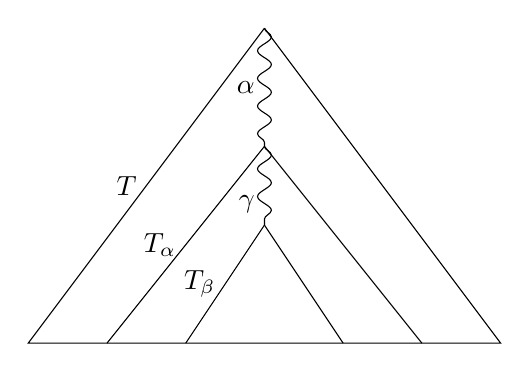
\begin{tikzpicture}
    \coordinate (A) at (0,0);
    \coordinate (B) at (-3,-4);
    \coordinate (C) at (3,-4);
    \coordinate (D) at (0,-1.5);
    \coordinate (E) at (-2,-4);
    \coordinate (F) at (2,-4);
    \coordinate (G) at (0,-2.5);
    \coordinate (H) at (-1,-4);
    \coordinate (I) at (1,-4);

    \draw (A) -- node[left]{$T$} (B) -- (C) -- (A);

    \draw (D) -- node[left]{$T_\alpha$}(E);
    \draw (D) -- (F);

    \draw (G) -- node[left]{$T_\beta$}(H);
    \draw (G) -- (I);

    \draw [photon] (A) -- node[left]{$\alpha$} (D);
    \draw [photon] (D) -- node[below left]{$\gamma$} (G);
  \end{tikzpicture}
\end{hint}

\begin{problem}
  Нека $P = (T,\lambda)$ и $P' = (T',\lambda')$ са дървета на извод съвместими с $G$ и нека
  \[\texttt{yield}(P) = \omega_1 \cdot \texttt{root}(P') \cdot \omega_2.\]
  Това означава, че съществува $\alpha$, за което $\lambda(\alpha) = \texttt{root}(P')$.

  Дефинираме $P'' = (T'',\lambda'')$ по следния начин:
  \begin{itemize}
  \item
    \marginpar{Ясно е, че $\alpha \in T$ и $\alpha \in \alpha\cdot T'$, но понеже $X_\alpha = X'_\varepsilon$, то нямаме проблем.}
    $T'' \df T \cup \alpha \cdot T'$;
  \item
    $\lambda''(\gamma) \df
    \begin{cases}
      \lambda(\gamma), & \text{ако }\gamma \in T\\
      \lambda'(\beta), & \text{ако }\beta \in \alpha \cdot T'\ \&\ \gamma = \alpha \cdot \beta.
    \end{cases}$
    
    Понеже $\alpha \in \texttt{front}(T)$ и $\lambda(\alpha) = \lambda'(\varepsilon)$, то функцията $\lambda''$ е коректно дефинирана.
  \end{itemize}
  Тогава $P''$ е дърво на извод съвместимо с $G$ и
  \[\texttt{yield}(P'') = \omega_1 \cdot \texttt{yield}(P') \cdot \omega_2.\]
  Нека в такъв случай да означаваме $P'' = P \odot P'$.
  
  \begin{figure}[htp]
    \begin{subfigure}[t]{0.5\textwidth}
      \centering
      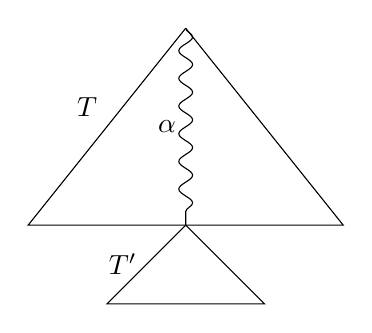
\begin{tikzpicture}
        \coordinate (A) at (0,0);
        \coordinate (B) at (-2,-2.5);
        \coordinate (C) at (2,-2.5);
        \coordinate (D) at (0,-2.5);
        \coordinate (E) at (-1,-3.5);
        \coordinate (F) at (1,-3.5);
        
        \draw (A) -- node[above left]{$T$} (B) -- (C) -- (A);
        \draw (D) -- node[left]{$T'$} (E) -- (F) -- (D);
        
        \draw [photon] (A) -- node[left]{$\alpha$} (D);
      \end{tikzpicture}
      \caption{Дървото $T''$}
      \end{subfigure}
      $\stackrel{\lambda}{\Rightarrow}$
      \begin{subfigure}[t]{0.5\textwidth}
        \centering
        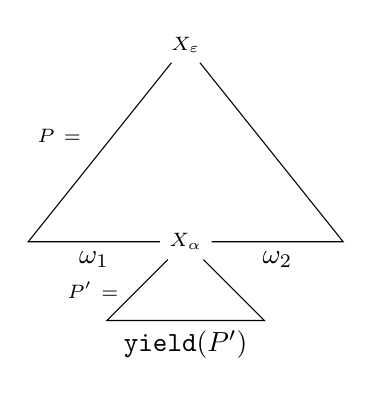
\begin{tikzpicture}
          \node (A) at (0,0) {${\scriptstyle X_\varepsilon}$};
          \coordinate (B) at (-2,-2.5);
          \coordinate (C) at (2,-2.5);
          \node (D) at (0,-2.5) {${\scriptstyle X_\alpha}$};
          \coordinate (E) at (-1,-3.5);
          \coordinate (F) at (1,-3.5);
          
          \draw (A) -- node[above left]{${\scriptstyle P\ =\ }$} (B) -- node[below]{$\omega_1$}(D) -- node[below]{$\omega_2$}(C) -- (A);
          \draw (D) -- node[left]{${\scriptstyle P'\ =\ }$}(E) -- node[below]{$\texttt{yield}(P')$}(F) -- (D);
          
          % \draw [photon] (A) -- node[left]{$\alpha$} (D);
        \end{tikzpicture}
        \caption{$P'' = P \odot P'$}
      \end{subfigure}
    \end{figure}
  \end{problem}
  
  Сега да разгледаме частния случай, когато $P = P'$. Тогава имаме, че $X_\varepsilon = X_\alpha$.
  Дефинираме $n$-тата степен на дървото $P$ по следния начин:
  \begin{itemize}
\item
  $P^{(0)} = (T_0,\lambda_0)$, където $T_0 = \{\varepsilon\}$ и $\lambda_0(\varepsilon) = \texttt{root}(P)$;
\item
  $P^{(n+1)} = P^{(n)} \odot P$.
\end{itemize}

\begin{problem}
  Докажете, че $P^{(n+k)} = P^{(n)} \odot P^{(k)}$.
\end{problem}

\begin{framed}
  \begin{problem}
    \label{prob:tree:iteration}
    Нека $\texttt{yield}(P) = \omega_1 \cdot \texttt{root}(P) \cdot \omega_2$.
    Докажете, че за всяко естествено число $i$,
    \[\texttt{yield}(P^{(i)}) = \omega^i_1 \cdot \texttt{root}(P) \cdot \omega^i_2.\]
  \end{problem}
\end{framed}
\begin{hint}
  Картинката за $i = 2$ изглежда така:

  \begin{figure}[htp]
    \begin{subfigure}[t]{0.5\textwidth}
      \centering
      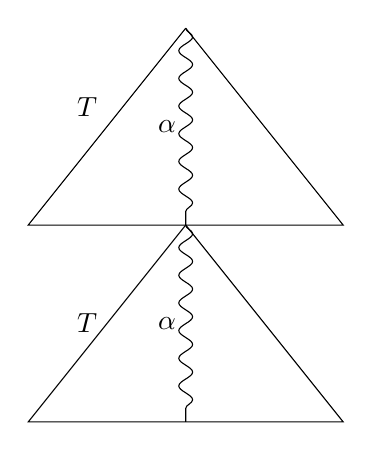
\begin{tikzpicture}
        \coordinate (A) at (0,0);
        \coordinate (B) at (-2,-2.5);
        \coordinate (C) at (2,-2.5);
        \coordinate (D) at (0,-2.5);
        \coordinate (E) at (-2,-5);
        \coordinate (F) at (2,-5);
        \coordinate (G) at (0,-5);
        
        \draw (A) -- node[above left]{$T$} (B) -- (C) -- (A);
        \draw (D) -- node[left]{$T$} (E) -- (F) -- (D);
        
        \draw [photon] (A) -- node[left]{$\alpha$} (D);
        \draw [photon] (D) -- node[left]{$\alpha$} (G);
      \end{tikzpicture}
      \caption{}
    \end{subfigure}
    $\stackrel{\lambda}{\Rightarrow}$
    \begin{subfigure}[t]{0.5\textwidth}
      \centering
      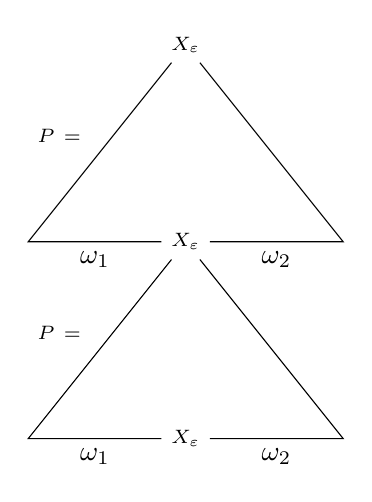
\begin{tikzpicture}
        \node (A) at (0,0) {${\scriptstyle X_\varepsilon}$};
        \coordinate (B) at (-2,-2.5);
        \coordinate (C) at (2,-2.5);
        \node (D) at (0,-2.5) {${\scriptstyle X_\varepsilon}$};
        \coordinate (E) at (-2,-5);
        \coordinate (F) at (2,-5);
        \node (G) at (0,-5) {${\scriptstyle X_\varepsilon}$};
        
        \draw (A) -- node[above left]{${\scriptstyle P\ =\ }$} (B) -- node[below]{$\omega_1$}(D) -- node[below]{$\omega_2$}(C) -- (A);
        \draw (D) -- node[above left]{${\scriptstyle P\ =\ }$}(E) -- node[below]{$\omega_1$} (G) -- node[below]{$\omega_2$} (F) -- (D);
      \end{tikzpicture}
      \caption{$\texttt{yield}(P^{(2)}) = \omega^2_1 \cdot \texttt{root}(P) \cdot \omega^2_2$}
    \end{subfigure}
  \end{figure}
\end{hint}

\begin{problem}
  Нека $P = (T,\lambda)$ е дърво на извод съвместимо с $G$ и $\alpha \in T$.
  Дефинираме $P \setminus P_\alpha = (T',\lambda')$ по следния начин:
  \begin{itemize}
  \item
    \marginpar{Съобразете, че $\alpha \in \texttt{front}(T')$.}
    $T' = T \setminus \{ \gamma \in T\mid \alpha \prec \gamma\}$;
  \item
    $\lambda'(\gamma) = \lambda(\gamma)$ за $\gamma \in T'$.
  \end{itemize}
  Докажете, че $P\setminus P_\alpha$ е дърво на извод съвместимо с $G$ и 
  \[P = (P\setminus P_\alpha) \odot P_\alpha.\]
\end{problem}
\begin{hint}
  Имаме следната картинка:

  \begin{figure}[htp]
    \begin{subfigure}[t]{0.5\textwidth}
      \centering
      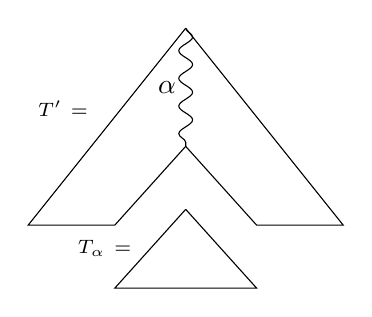
\begin{tikzpicture}
        \coordinate (A) at (0,0);
        \coordinate (B) at (-2,-2.5);
        \coordinate (C) at (2,-2.5);
        \coordinate (D) at (-0.9,-2.5);
        \coordinate (E) at (0.9,-2.5);
        \coordinate (F) at (0,-1.5);
        
        \coordinate (G) at (0,-2.3);
        \coordinate (H) at (-0.9,-3.3);
        \coordinate (I) at (0.9,-3.3);
        
        \draw (A) -- node[above left]{${\scriptstyle T'\ =\ }$}(B) -- (D) -- (F) -- (E) -- (C) -- (A);
        \draw (G) -- node[left]{${\scriptstyle T_\alpha\ =\ }$} (H) -- (I) -- (G);
        
        \draw [photon] (A) -- node[left]{$\alpha$} (F);
      \end{tikzpicture}
      \caption{$T_\alpha = \alpha^{-1}(T)$}
    \end{subfigure}
    $\stackrel{\lambda}{\Rightarrow}$
    \begin{subfigure}[t]{0.5\textwidth}
      \centering
      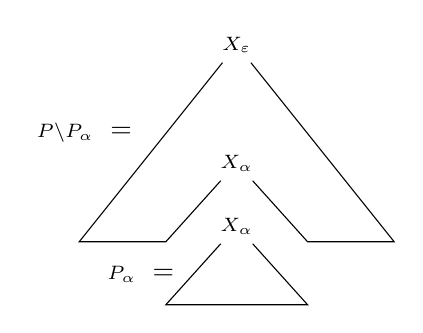
\begin{tikzpicture}
        \node (A) at (0,0) {${\scriptstyle X_\varepsilon}$};
        \coordinate (B) at (-2,-2.5);
        \coordinate (C) at (2,-2.5);
        \coordinate (D) at (-0.9,-2.5);
        \coordinate (E) at (0.9,-2.5);
        \node (F) at (0,-1.5) {${\scriptstyle X_\alpha}$};
        
        \node (G) at (0,-2.3) {${\scriptstyle X_\alpha}$};
        \coordinate (H) at (-0.9,-3.3);
        \coordinate (I) at (0.9,-3.3);
        
        \draw (A) -- node[above left]{${\scriptstyle P\setminus P_\alpha}\ =\ $}(B) -- (D) -- (F) -- (E) -- (C) -- (A);
        \draw (G) -- node[left]{${\scriptstyle P_\alpha}\ =\ $} (H) -- (I) -- (G);
      \end{tikzpicture}
      \caption{$\texttt{yield}(P\setminus P_\alpha) = \omega_1 \cdot \texttt{root}(P_\alpha) \cdot \omega_2$}
    \end{subfigure}
  \end{figure}
\end{hint}


\subsection*{Ляв извод в граматика}

В нашата дефиниция на извод, изборът върху коя променлива да приложим правило от граматиката е недетерминистичен.
В някои случаи, за нас ще бъде важно винаги да правим детерминистичен избор на това върху коя променлива прилагаме правило.

За две думи $\alpha,\beta \in (V\cup\Sigma)^\star$, дефинираме {\bf ляв извод} в граматиката $G$, $\alpha \to_{G,\texttt{L}} \beta$,  по следния начин:
ако $\alpha = \alpha_1A\alpha_2$ и $\alpha_1 \in \Sigma^\star$, $A \to_G \gamma$ е правило в граматиката $G$, то
$\beta = \alpha_1\gamma \alpha_2$.

Както преди, с $\to^\star_{G,\texttt{L}}$ ще означаваме рефлексивното и транзитивно затваряне на релацията $\to_{G,\texttt{L}}$.

Ясно е, че ако $\alpha \to^\star_{G,\texttt{L}} \beta$, то $\alpha \to^\star_G \beta$.
Да видим защо имаме и обратната посока.

Очевидно е, че ако $\alpha \to^\star_{G,\texttt{L}} \beta$, то $\alpha \to^\star_G \beta$.
Това означава, че ако $X \to^\star_{G,\texttt{L}} \beta$, то същестува дърво на извод с корен $X$ за думата $\beta$.

\begin{lemma}
  Нека $P = (T,\lambda)$ е дърво на извод за думата $\beta \in (V\cup\Sigma)^\star$ в $G$.
  Тогава $X_\varepsilon \to^\star_{G,\texttt{L}} \beta$.
\end{lemma}  
\begin{hint}
  Индукция по $\texttt{height}(T)$.
\end{hint}



%%% Local Variables:
%%% mode: latex
%%% TeX-master: "../eai"
%%% End:
